\section{Introduction}

Flying vehicles remain an active research domain for the Robotics community after decades of studies in the subject. 
For instance, inspection via \emph{passive} Vertical Take Off and Landing (VTOL) systems and grasping and manipulation using \emph{active} flying vehicles represent   research problems that still call for new tools and methods \cite{c8,c9,c10}. Often, the control of \emph{small} aircraft neglects the aerodynamic effects acting on the body, which is a barrier for improving the vehicle performance and flight envelope \cite{c11,c13}. This paper proposes an approach that considers advanced aerodynamic modelling techniques for the conception of simplified  models then used on-line for the control of flying multibody robots.

The problem of flying vehicle control is especially challenging for the so-called multimodal robots, which attempt at combining terrestrial and aerial locomotion in a single robotic platform. Hexapod-quadrotors, insect biobots, and humanoid robots with thrusters are examples of platforms that combine different degrees of locomotion, thus requiring advanced control and modeling methods \cite{pitonyak2017hexapod,kalantari2013hytaq,bozkurt2009insectbio,LeoCaltech,Jet-HR1}. In this category of platforms there is iRonCub, a prototype of flying humanoid robot currently developed at the Italian Institute of Technology~\cite{c1,c2,Giuse,9622189}.~As shown in Fig.~\ref{fig:iron_cad}, four jet engines located on the robot arms and chest are used to lift from the ground a reworked version of the longstanding iCub platform \cite{Bartolozzi2017iCubTN}.

\begin{figure}[t]
      \centering
%      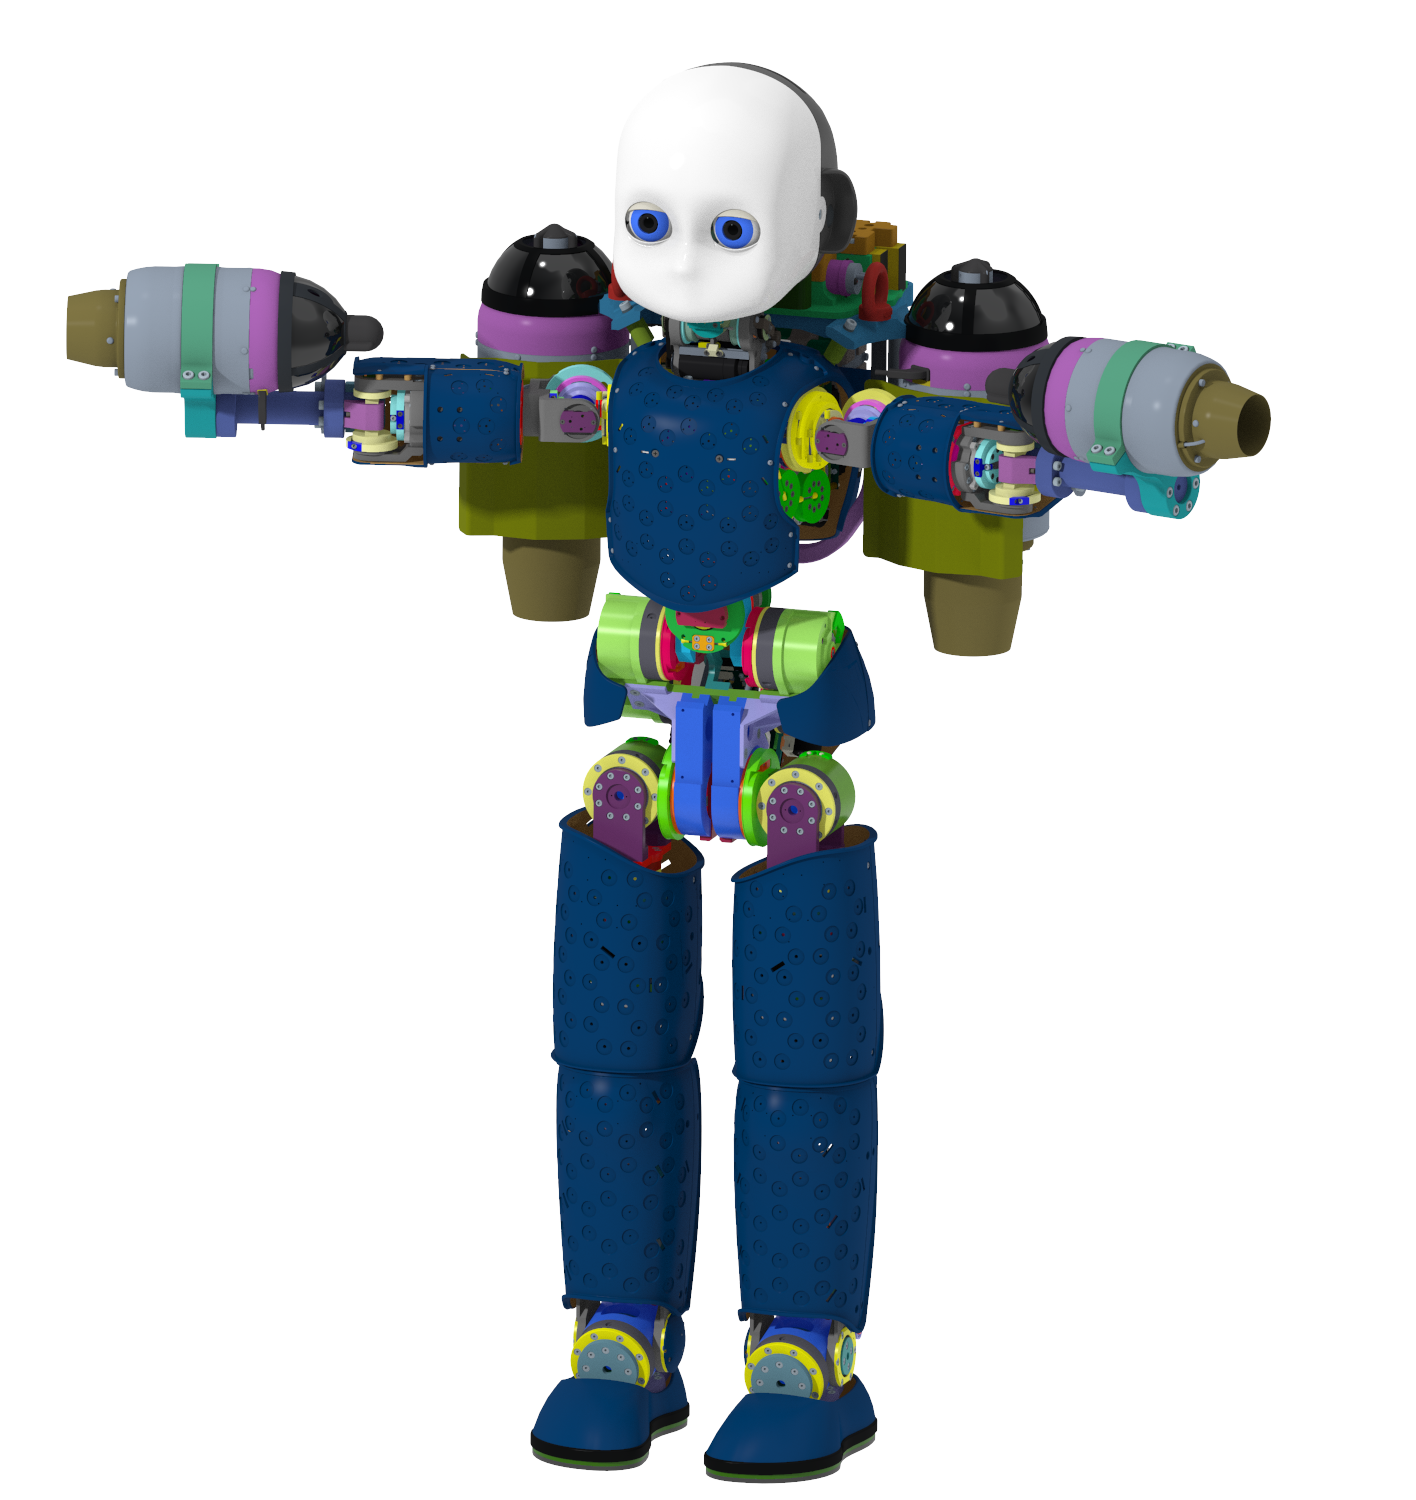
\includegraphics[width=55mm]{./imagines/mk1-5.png}
      
\includegraphics[width=0.7\columnwidth]{./imagines/ironcub.png}
      \caption{The jet-powered humanoid robot iRonCub.}
      \label{fig:iron_cad}
\end{figure}

A common assumption for high DoF VTOL systems is that the vehicle operates at relatively \emph{small speed}, often in indoor environments \cite{c8,c9,c10}, and  consequently the aerodynamic forces acting on the system are usually negligible and not considered in modeling and control framework \cite{c11,c28}. When aerodynamic effects are important enough to affect system stability during flight, or high precision is required for performing a task, different modeling and control strategies could be adopted, e.g. to estimate aerodynamic force by designing a momentum-based observer or other disturbances estimation strategies \cite{c17,c16} and to compensate estimated aerodynamic force by means of adaptive control strategies \cite{c14,c15}. However, the absence of an explicit model of the aerodynamic forces could impair the effectiveness of these methods for exploiting physical properties that are beneficial for flight.\looseness=-1

High-speed flight can benefit from the presence of lift forces alleviating the effort made by the propellers for gravity compensation. The VTOL dynamical model, in this case, explicitly includes aerodynamic forces \cite{c3,c18,KAI2019108491}. Few examples include the analysis of blade flapping on quadrotors, modeling first-order aerodynamic effects and evaluating the effect of drag force on thrust power under hovering, \cite{c7}\cite{c20}\cite{c19}. However, the shape of aerial vehicles has a significant role in modeling aerodynamics effects. It is difficult to design an effective aerodynamic model in case of complex-shaped, high DoF aerial systems \cite{c6,c18}.

Different techniques have been developed to properly estimate aerodynamic forces for complex-shaped systems, e.g. wind tunnel test and Computational Fluid Dynamics (CFD) analysis. However, to estimate the aerodynamic forces for an entire set of robot operating conditions, i.e. \emph{flight envelope}, it requires to collect a very large number of data. An alternative is to design simpler analytical models via limited dataset provided by wind tunnel tests or CFD simulations. Many of these analytical models assume that the robot body is axisymmetric \cite{c3,c23,c25}.

This paper proposes a framework to include aerodynamic forces in the modeling and control design of high DoF VTOL systems, which in the case under study are represented by the flying humanoid robot iRonCub. At first, a series of CFD simulations is performed on a simplified robot model, in order to generate a dataset of the aerodynamic forces acting on the robot for a given flight envelope. Secondly, a model for a non-axisymmetric bluff body is designed to fit the collected dataset and estimate the aerodynamic characteristics in between the flight envelope. Finally, the model is used to improve the iRonCub flight-control strategy developed in our previous works \cite{c1}\cite{c2} by compensation of the aerodynamic forces via \emph{feedback linearization} and improvement of the controller robustness with \emph{gain scheduling}.

The paper is organized as follows. Sec.~\ref{background} recalls notation, system modeling and fundamentals of aerodynamic modeling. In Sec.~\ref{methods}, we describe the CFD analysis on a simplified iRonCub model and the identification of the aerodynamic characteristics. Sec.~\ref{sec:control} presents the improvements of iRonCub flight controller to handle aerodynamic effects. Simulation results are displayed in Sec.~\ref{simulation}. Sec.~\ref{conclusion} concludes the paper and points out future directions.

